
\section{SR reachability}

\begin{definition}
A sr-path $\sr{p} = \langle x_1, \ldots, x_k \rangle$ on a network $G$ is said to be \emph{deterministic}
iff for each $i = 2, \ldots, k$ there is a unique IGP shortest path between $x^2_{i - 1}$ and $x^1_i$.
\end{definition}

Deterministic sr-paths are interesting in the context of network monitoring because, as they do not use ECMP,
we can know exactly which edges are traversed by packets forwarded on them. This allows to know whether
all links in the network are covered by a set of sr-paths or not.

Figure \ref{fig:non-ecmp-free} illustrates the sr-path $\langle \node{a}, \node{b}, (\node{d}, \node{g}, 0), \node{j} \rangle$.
This sr-path is not deterministic because between $x^2_1 = \node{b}$ and $x^1_2 = \node{d}$ there are two shortest paths, namely,
$(\node{b}, \node{c}, \node{d})$ and $(\node{b}, \node{e}, \node{d})$. This means that there is underctainty about the set of 
edges covered by this path. If we were to use this path in an edge
covering of the network, only edges $(\node{a}, \node{b}), (\node{d}, \node{g}, 0), (\node{g}, \node{h})$ and $(\node{h}, \node{j})$
would be guaranteed to be covered by it.

\begin{figure}[H]
\begin{center}
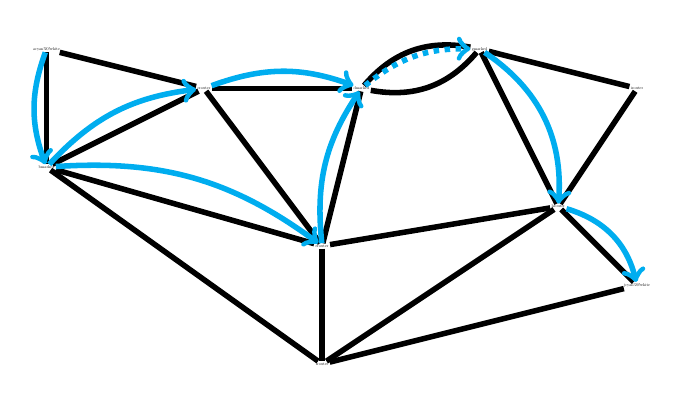
\begin{tikzpicture}
\def\x{0}
\def\y{0}
\node[scale=0.15] (a) at (0.5 + \x,  0.5 + \y) {\router{a}{cyan!20!white}};
\node[scale=0.15] (b) at (0.5 + \x, -1.0 + \y) {\router{b}{marked}};
\node[scale=0.15] (c) at (2.5 + \x,  0.0 + \y) {\router{c}{router}};
\node[scale=0.15] (d) at (4.5 + \x,  0.0 + \y) {\router{d}{marked}};
\node[scale=0.15] (e) at (4.0 + \x, -2.0 + \y) {\router{e}{router}};
\node[scale=0.15] (g) at (6.0 + \x,  0.5 + \y) {\router{g}{marked}};
\node[scale=0.15] (i) at (8.0 + \x,  0.0 + \y) {\router{i}{router}};
\node[scale=0.15] (h) at (7.0 + \x, -1.5 + \y) {\router{h}{router}};
\node[scale=0.15] (f) at (4.0 + \x, -3.5 + \y) {\router{f}{router}};
\node[scale=0.15] (j) at (8.0 + \x, -2.5 + \y) {\router{j}{cyan!20!white}};
\draw[line width=2] (f) edge[above, sloped] node[black,font=\bfseries] {\tiny \texttt{}} (j);
\draw[line width=2] (h) edge[above, sloped] node[black,font=\bfseries] {\tiny \texttt{}} (j);
\draw[line width=2] (a) edge[above, sloped] node[black,font=\bfseries] {\tiny \texttt{}} (b);
\draw[line width=2] (b) edge[above, sloped] node[black,font=\bfseries] {\tiny \texttt{}} (c);
\draw[line width=2] (e) edge[above, sloped] node[black,font=\bfseries] {\tiny \texttt{}} (c);
\draw[line width=2] (b) edge[above, sloped] node[black,font=\bfseries] {\tiny \texttt{}} (e);
\draw[line width=2] (b) edge[above, sloped] node[black,font=\bfseries] {\tiny \texttt{}} (f);
\draw[line width=2] (e) edge[above, sloped] node[black,font=\bfseries] {\tiny \texttt{}} (f);
\draw[line width=2] (h) edge[above, sloped] node[black,font=\bfseries] {\tiny \texttt{}} (f);
\draw[line width=2] (g) edge[above, sloped] node[black,font=\bfseries] {\tiny \texttt{}} (i);
\draw[line width=2] (i) edge[above, sloped] node[black,font=\bfseries] {\tiny \texttt{}} (h);
\draw[line width=2]  (d) edge[above, sloped, bend left] node[black,font=\bfseries] {\tiny \texttt{}} (g);
\draw[line width=2]  (d) edge[above, sloped, bend right] node[black,font=\bfseries] {\tiny \texttt{}} (g);
\draw[line width=2]  (d) edge[above, sloped] node[black,font=\bfseries] {\tiny \texttt{}} (e);
\draw[line width=2]  (e) edge[above, sloped] node[black,font=\bfseries] {\tiny \texttt{}} (h);
\draw[line width=2]  (g) edge[above, sloped] node[black,font=\bfseries] {\tiny \texttt{}} (h);
\draw[line width=2]  (c) edge[above, sloped] node[black,font=\bfseries] {\tiny \texttt{}} (d);
\draw[line width=2]  (a) edge[above, sloped] node[black,font=\bfseries] {\tiny \texttt{}} (b);
\draw[line width=2]  (a) edge[above, sloped] node[black,font=\bfseries] {\tiny \texttt{}} (c);

%%%%
\draw (a) edge[line width=2, cyan, above, ->, bend right = 20] (b);
\draw (b) edge[line width=2, cyan, above, ->, bend left = 20] (c);
\draw (b) edge[line width=2, cyan, above, ->, bend left = 20] (e);
\draw (c) edge[line width=2, cyan, above, ->, bend left = 20] (d);
\draw (e) edge[line width=2, cyan, above, ->, bend left = 20] (d);

\draw (d) edge[line width=2, cyan, above, ->, bend left = 20, bend left, dotted] (g);
\draw (g) edge[line width=2, cyan, above, ->, bend left] (h);
\draw (h) edge[line width=2, cyan, above, ->, bend left] (j);

\end{tikzpicture}
\end{center}
\label{fig:non-ecmp-free}
\caption{An example of a sr-path that is not deterministic.}
\end{figure}

On the other hand, the sr-path $\langle \node{a}, (\node{d}, \node{g}, 0), \node{j} \rangle$ shown in Figure \ref{fig:ecmp-free} is deterministic. There
is no uncertainty about the set of edges covered by this path, we are sure that
if covers edges $(\node{a}, \node{c}), (\node{c}, \node{d}), (\node{d}, \node{g}, 0), (\node{g}, \node{h})$ and $(\node{h}, \node{j})$. 

\begin{figure}[H]
\begin{center}
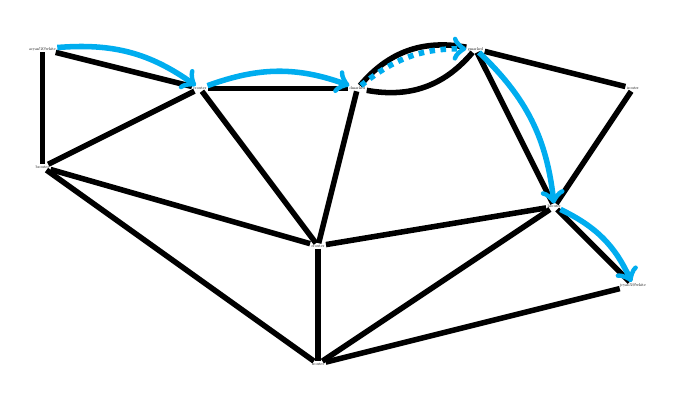
\begin{tikzpicture}
\def\x{0}
\def\y{0}
\node[scale=0.15] (a) at (0.5 + \x,  0.5 + \y) {\router{a}{cyan!20!white}};
\node[scale=0.15] (b) at (0.5 + \x, -1.0 + \y) {\router{b}{router}};
\node[scale=0.15] (c) at (2.5 + \x,  0.0 + \y) {\router{c}{router}};
\node[scale=0.15] (d) at (4.5 + \x,  0.0 + \y) {\router{d}{marked}};
\node[scale=0.15] (e) at (4.0 + \x, -2.0 + \y) {\router{e}{router}};
\node[scale=0.15] (g) at (6.0 + \x,  0.5 + \y) {\router{g}{marked}};
\node[scale=0.15] (i) at (8.0 + \x,  0.0 + \y) {\router{i}{router}};
\node[scale=0.15] (h) at (7.0 + \x, -1.5 + \y) {\router{h}{router}};
\node[scale=0.15] (f) at (4.0 + \x, -3.5 + \y) {\router{f}{router}};
\node[scale=0.15] (j) at (8.0 + \x, -2.5 + \y) {\router{j}{cyan!20!white}};
\draw[line width=2] (f) edge[above, sloped] node[black,font=\bfseries] {\tiny \texttt{}} (j);
\draw[line width=2] (h) edge[above, sloped] node[black,font=\bfseries] {\tiny \texttt{}} (j);
\draw[line width=2] (a) edge[above, sloped] node[black,font=\bfseries] {\tiny \texttt{}} (b);
\draw[line width=2] (b) edge[above, sloped] node[black,font=\bfseries] {\tiny \texttt{}} (c);
\draw[line width=2] (e) edge[above, sloped] node[black,font=\bfseries] {\tiny \texttt{}} (c);
\draw[line width=2] (b) edge[above, sloped] node[black,font=\bfseries] {\tiny \texttt{}} (e);
\draw[line width=2] (b) edge[above, sloped] node[black,font=\bfseries] {\tiny \texttt{}} (f);
\draw[line width=2] (e) edge[above, sloped] node[black,font=\bfseries] {\tiny \texttt{}} (f);
\draw[line width=2] (h) edge[above, sloped] node[black,font=\bfseries] {\tiny \texttt{}} (f);
\draw[line width=2] (g) edge[above, sloped] node[black,font=\bfseries] {\tiny \texttt{}} (i);
\draw[line width=2] (i) edge[above, sloped] node[black,font=\bfseries] {\tiny \texttt{}} (h);
\draw[line width=2]  (d) edge[above, sloped, bend left] node[black,font=\bfseries] {\tiny \texttt{}} (g);
\draw[line width=2]  (d) edge[above, sloped, bend right] node[black,font=\bfseries] {\tiny \texttt{}} (g);
\draw[line width=2]  (d) edge[above, sloped] node[black,font=\bfseries] {\tiny \texttt{}} (e);
\draw[line width=2]  (e) edge[above, sloped] node[black,font=\bfseries] {\tiny \texttt{}} (h);
\draw[line width=2]  (g) edge[above, sloped] node[black,font=\bfseries] {\tiny \texttt{}} (h);
\draw[line width=2]  (c) edge[above, sloped] node[black,font=\bfseries] {\tiny \texttt{}} (d);
\draw[line width=2]  (a) edge[above, sloped] node[black,font=\bfseries] {\tiny \texttt{}} (b);
\draw[line width=2]  (a) edge[above, sloped] node[black,font=\bfseries] {\tiny \texttt{}} (c);

%%%%
\draw (a) edge[line width=2, cyan, above, ->, bend left = 20] (c);
\draw (c) edge[line width=2, cyan, above, ->, bend left = 20] (d);
\draw (d) edge[line width=2, cyan, above, ->, bend left = 20, bend left, dotted] (g);
\draw (g) edge[line width=2, cyan, above, ->, bend left = 20] (h);
\draw (h) edge[line width=2, cyan, above, ->, bend left = 20] (j);

\end{tikzpicture}
\end{center}
\label{fig:ecmp-free}
\caption{An example of a sr-path that is deterministic.}
\end{figure}

\begin{problem}{Single point sr-path network covering}
\label{problem:networkcover}
\textbf{Input:} A network $G$.

\textbf{Output:} A node $v \in V(G)$ and set of deterministic sr-paths $\sr{p}_1, \ldots, \sr{p}_k$ from $v$ to $v$
such that for each edge $e \in E(G)$ there exists $i$ such that $e \in E(\sr{p}_i)$.
\end{problem}

The formulation of the Problem \ref{problem:networkcover} is quite general as it does not impose any constraints on the
number $k$ of paths in the solution or the segment cost of these paths. In practice we want both of these to be as small as possible.
If we have a low number of paths to cover the network, less probes are necessary to monitor link failures and so monitoring
incurs less overhead on the network. Having paths with low segment cost is a necessity due to hardware limitations of the routers. 
These two objectives are somewhat conflicting since to have a low amout of paths covering the entire network we likely need to use
very long paths and the longer a path is the more likely we are to need a high amout of segments to represent the path.

\todo{related work about cycle covering}

\section{Lower bounds on the segment cost}

Before we proceed with presenting our solutions to Problem \ref{problem:networkcover}, we will see that we can actually compute
a lower bound for each given network on the number of segments required to cover a network from a single vantage point with deterministic
sr-paths. For this, we first need to define some new theory.

\begin{definition}
Let $G$ be a network and $v \in V(G)$. We define
\begin{align*}
\nreach(v, k) = & \ \textrm{set of nodes $u \in V(G)$ such that there exists a deterministic} \\ 
                & \ \textrm{sr-path $\sr{p}$ from $v$ to $u$ of segment cost at most $k$}
\end{align*}
and
\begin{align*}
\ereach(v, k) = & \ \textrm{set of edges $e \in E(G)$ such that there exists a deterministic} \\ 
                & \ \textrm{sr-path of segment cost at most $k$, $\sr{p} = \langle x_1, \ldots, x_{l - 1}, x_l \rangle$,} \\
                & \ \textrm{from $v$ to $u_2$ such that either $e = x_l$ or $x_l$ is a node segment} \\
                & \ \textrm{and $e$ is the last edge of the unique shortest path between $x^2_{l - 1}$} \\
                & \ \textrm{and $x_l$}
\end{align*}
\end{definition}

Intuitively, these definitions are saying that $\nreach(v, k)$ is the set of nodes that
we can reach using a sr-path of cost at most $k$ from $v$ and $\ereach(v, k)$ is the
set of edges that we can cover using a sr-path of cost at most $k$ from $v$.

We denote the minimum $k$ for which there exists $v \in V(G)$ such that $\nreach(v, k) = V(G)$ as $\kn(G)$. 
Similarly, the minium $k$ such that for some $v \in V(G)$ it holds that $\ereach(v, k) = E(G)$ is denoted by $\ke(G)$.

\begin{proposition}
Let $G$ be a strongly connected network. Then, $\kn(G)$ and $\ke(G)$ are always well defined and $\kn(G), \ke(G) \leq 2 \cdot |E(G)|$.
\end{proposition}

\begin{proof}
Let $v \in V(G)$ by any node of $G$. Let $u \in V(G)$. Since $G$ is strongly connected, there exists a simple path $p_u = (e_1, e_2, \ldots, e_{l_u})$ on $G$ from $v$ to $u$.
Then the sr-path $\sr{p} = \langle e_1, e_2, \ldots, e_{l_u} \rangle$ is a deterministic sr-path from $v$ to $u$ with segments cost
$2 \cdot l_u$. Thus $\kn(G) \leq \max_{u \in V(G)} \ 2 \cdot l_u \leq 2 \cdot |E(G)|$.

Let $f = (u_1, u_2) \in E(G)$. Since $G$ is strongly conencted, there exists a simple path $p_f = (e_1, e_2, \ldots, e_{l_f})$ on $G$ from
$v$ to $u_1$. Thus the sr-path $\sr{p} = \langle e_1, e_2, \ldots, e_{l_f}, f \rangle$ is a deterministic sr-path from $v$ to $u_2$ of
segment cost $2 \cdot (l_f + 1) \leq 2 \cdot |E(G)|$ since $p_f$ is simple. Therefore $\ke(G) \leq \max_{f \in E(G)} \ 2 \cdot (l_f + 1) \leq 2 \cdot |E(G)|$.
\end{proof}

Computing $\ke(G)$ gives us a lower bound on the maximum segment cost of any sr-path in a solution of Problem \ref{problem:networkcover}.
We propose a polynomial time algorithm for computing $\ke(G)$ and run it on every topology in our data set
to analyse the segment cost that we can expect to have on the worst case.

\subsubsection*{Computing $\nreach(v, k)$ and $\ereach(v, k)$}

In order to compute $\nreach(v, k)$ we will express it recursivelly in terms of smaller values of $k$ and then
use dynamic programming to compute it for all $v$ and relevant $k$.

Computing $\nreach(v, 0)$ is trivial. For each $v$, the only node that is reachable using a path of segment cost $0$ is the empty path.
Therefore $\nreach(v, 0) = \{ v \}$ for all $v \in V(G)$. For $k = 1$ the problem can easily be solved using Dijkstra's algorithm.
To compute $\nreach(v, 1)$ we execute Dijkstra starting from node $v$ in order to compute $\sp(v)$, the shortest path DAG rooted at node
$v$. From $\sp(v)$ we want to extract all nodes $u$ for which there exists a unique path starting at $v$. This can be achieved in linear time
with a breadth-first search on $\sp(V)$ starting at node $v$ and only adding nodes with in-degree $1$ to the queue.

Figure \ref{fig:reach1} illustrates this process for $v = \node{a}$. The blue edges show the edges that belong to $\sp(V)$. The shaded region 
contains the nodes in $\nreach(\node{a}, 1)$.

\begin{figure}[H]
\begin{center}
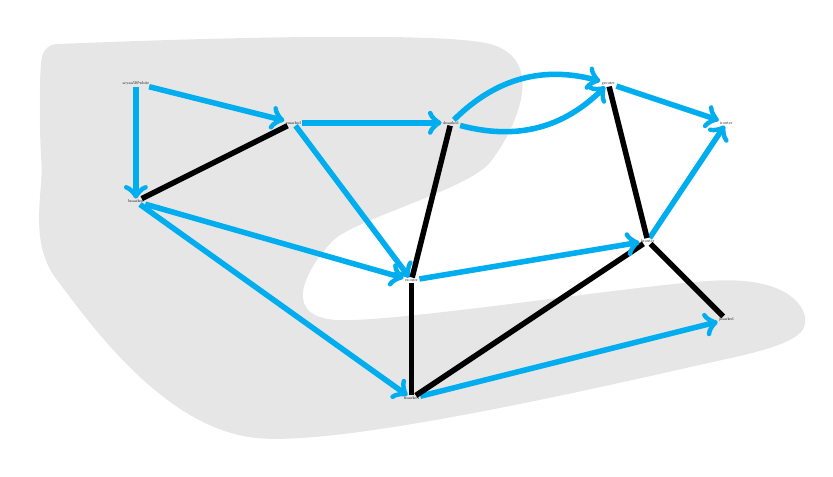
\begin{tikzpicture}
\def\x{0}
\def\y{0}

\fill[gray, opacity = 0.2] plot [smooth] coordinates { (-0.5, 1) (5, 1) (5, -0.5) (3, -1.5) (3, -2.5) (8, -2) (9, -2.5) (8, -3) (2, -4) (-0.5, -2) (-0.7, -0.5) (-0.7, 0.8) (-0.5, 1)};

\node[scale=0.15] (a) at (0.5 + \x,  0.5 + \y) {\router{a}{cyan!20!white}};
\node[scale=0.15] (b) at (0.5 + \x, -1.0 + \y) {\router{b}{marked}};
\node[scale=0.15] (c) at (2.5 + \x,  0.0 + \y) {\router{c}{marked}};
\node[scale=0.15] (d) at (4.5 + \x,  0.0 + \y) {\router{d}{marked}};
\node[scale=0.15] (e) at (4.0 + \x, -2.0 + \y) {\router{e}{router}};
\node[scale=0.15] (g) at (6.5 + \x,  0.5 + \y) {\router{g}{router}};
\node[scale=0.15] (i) at (8.0 + \x,  0.0 + \y) {\router{i}{router}};
\node[scale=0.15] (h) at (7.0 + \x, -1.5 + \y) {\router{h}{router}};
\node[scale=0.15] (f) at (4.0 + \x, -3.5 + \y) {\router{f}{marked}};
\node[scale=0.15] (j) at (8.0 + \x, -2.5 + \y) {\router{j}{marked}};
\draw[line width=2] (f) edge[above, sloped, ->, cyan] node[black,font=\bfseries] {\tiny \texttt{}} (j);
\draw[line width=2] (h) edge[above, sloped] node[black,font=\bfseries] {\tiny \texttt{}} (j);
\draw[line width=2] (b) edge[above, sloped] node[black,font=\bfseries] {\tiny \texttt{}} (c);
\draw[line width=2] (c) edge[above, sloped, ->, cyan] node[black,font=\bfseries] {\tiny \texttt{}} (e);
\draw[line width=2] (b) edge[above, sloped, ->, cyan] node[black,font=\bfseries] {\tiny \texttt{}} (e);
\draw[line width=2] (b) edge[above, sloped, ->, cyan] node[black,font=\bfseries] {\tiny \texttt{}} (f);
\draw[line width=2] (e) edge[above, sloped] node[black,font=\bfseries] {\tiny \texttt{}} (f);
\draw[line width=2] (h) edge[above, sloped] node[black,font=\bfseries] {\tiny \texttt{}} (f);
\draw[line width=2] (g) edge[above, sloped, ->, cyan] node[black,font=\bfseries] {\tiny \texttt{}} (i);
\draw[line width=2] (h) edge[above, sloped, ->, cyan] node[black,font=\bfseries] {\tiny \texttt{}} (i);
\draw[line width=2] (d) edge[above, sloped, bend left, ->, cyan] node[black,font=\bfseries] {\tiny \texttt{}} (g);
\draw[line width=2] (d) edge[above, sloped, bend right, ->, cyan] node[black,font=\bfseries] {\tiny \texttt{}} (g);
\draw[line width=2] (d) edge[above, sloped] node[black,font=\bfseries] {\tiny \texttt{}} (e);
\draw[line width=2] (e) edge[above, sloped, ->, cyan] node[black,font=\bfseries] {\tiny \texttt{}} (h);
\draw[line width=2] (g) edge[above, sloped] node[black,font=\bfseries] {\tiny \texttt{}} (h);
\draw[line width=2] (c) edge[above, sloped, ->, cyan] node[black,font=\bfseries] {\tiny \texttt{}} (d);
\draw[line width=2] (a) edge[above, sloped, ->, cyan] node[black,font=\bfseries] {\tiny \texttt{}} (b);
\draw[line width=2] (a) edge[above, sloped, ->, cyan] node[black,font=\bfseries] {\tiny \texttt{}} (c);

%%%%


\end{tikzpicture}
\end{center}
\label{fig:reach1}
\caption{$\nreach(\node{a}, 1)$ show as the colored nodes. The blue edges represent $\sp(\node{a})$.}
\end{figure}

We will now prove some results that will enable us to define
$\nreach(v, k)$ for $k \geq 2$ recursivelly and ultimatelly provide
an efficient algorithms for computing it. We start by a simple lemma
about the concateation of deterministic sr-paths.

\todo{define the concatenation, if the last element of p and q are both node segments,
keep only one of them, if they are both adjacency segments keep both otherwise keep
only the adjacency. this should be in the SR chapter}

\begin{lemma}
\label{lemma:deterministic-concat}
Let $G$ be a netwrok and $\sr{p}$ be a deterministic sr-path from
$x$ to $y$ with $\cost(\sr{p}) = k_1$
and $\sr{q}$ be a deterministic sr-path from $y$ to $z$ with 
$\cost(\sr{q}) = k_2$ then $\sr{p} \oplus \sr{q}$ is a deterministic sr-path
from $x$ to $z$ with segment cost $k_1 + k_2$.
\end{lemma}

\begin{proof}
Write $\sr{p} = \langle x_1, \ldots, x_l \rangle$ and 
$\sr{q} = \langle y_1, \ldots, y_r \rangle$.
Let $z_i, z_{i + 1}$ be consecutive elements of $\sr{p} \oplus \sr{q}$. 
We need to prove that
there exists a unique shortest path between $z^2_i$ and $z^1_{i + 1}$.
If both $z_i, z_{i + 1}$ belong to $\sr{p}$ or $\sr{q}$ then this is true since both
$\sr{p}$ and $\sr{q}$ are deterministic. Otherwise, there are four cases that we need
to consider.

\emph{Case 1:} $x_l = y_1$ are both node segments. In this case we know that
$\sr{p} \oplus \sr{q} = \langle x_1, \ldots, x_l, y_2, \ldots, y_r \rangle$.
Thus, $z_i = x_l = y_1$ and $z_{i + 1} = y_2$. Thus, since $\sr{q}$ is deterministic,
there exists a unique shortest path between $z^2_i = y^2_1$ and $z^1_{i + 1} = y^1_2$.

\emph{Case 2:} $x_l,  y_1$ are both adjacency segments and 
$x^2_l = y^1_1$. In this case we know that
$\sr{p} \oplus \sr{q} = \langle x_1, \ldots, x_l, y_1, y_2, \ldots, y_r \rangle$.
Hence, $z_i = x_l$ and $z_{i + 1} = y_1$ so $z^2_i = x^2_l = y^1_1 = z^1_{i + 1}$ so
the unique shortst path between $z^2_i$ and $z^1_{i + 1}$ is the empty path.

\emph{Case 3:} $x_l$ is an adjacency segment and $y_1$ is a node segment such that
$x^2_l = y_1$. By definition, 
$\sr{p} \oplus \sr{q} = \langle x_1, \ldots, x_l, y_2, \ldots, y_r \rangle$.
Thus, $z_i = x_l$ and $z_{i + 1} = y_2$. Thus, since $\sr{q}$ is deterministic,
there exists a unique shortest path between $z^2_i = x^2_l = y^2_1$ and $z^1_{i + 1} = y^1_2$.

\emph{Case 4:} $x_l$ is a node segment and $y_1$ is an adjacent segment such that
$y^1_l = x_l$. Therefore $\sr{p} \oplus \sr{q} = \langle x_1, \ldots, x_{l - 1}, y_1, y_2, \ldots, y_r \rangle$.
Thus, $z_i = x_{l - 1}$ and $z_{i + 1} = y_1$. Thus, since $\sr{p}$ is deterministic,
there exists a unique shortest path between $z^2_i = x^2_{l - 1}$ and $z^1_{i + 1} = y^1_2 = x^1_l$.

In each case the result holds so we have proved that $\sr{p} \oplus \sr{q}$ is
deterministic. The fact that its cost is $k_1 + k_2$ was already shown on Lemma 
\ref{lemma:contact}. \todo{make this lemma in sr chapter}
\end{proof}

We can now prove a recurrence expressing $\nreach(v, k)$ in terms of
$\nreach(v, k - 1)$. Let us build some intuition before proving it formally.

First, $\nreach(v, k)$ must contain any node $x$ for which there exists some node $u$ that is reachable using a deterministic sr-path of cost at 
most $k - 1$ such that $x$ is reachable with deterministic sr-path of cost $1$ from $u$. When this is the case we can concatenate
both sr-paths to obtain a deterministic sr-path from $v$ to $u$ as show in Figure \ref{fig:nreachC1}. More formally, we are saying that
$\nreach(v, k)$ contains all the nodes in

$$
\bigcup_{u \in \nreach(v, k - 1)} \nreach(u, 1).
$$

\begin{figure}
\begin{center}
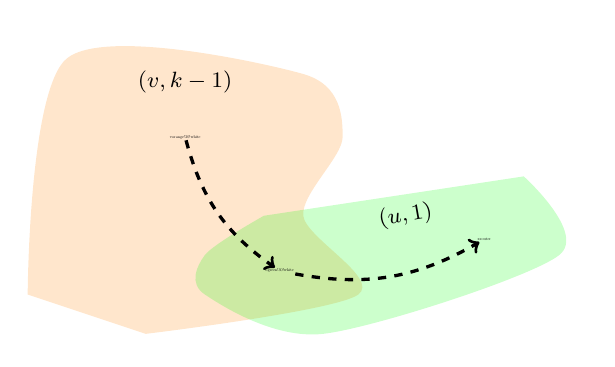
\begin{tikzpicture}
\fill[orange, opacity = 0.2] plot [smooth] coordinates { 
(-1.5, -1) 
(-1, 2) 
(2, 1.8) 
(2.5, 1) 
(2, 0) 
(2.7, -1) 
(0, -1.5)
};

\fill[green, opacity = 0.2, xscale = 1.5] plot [smooth] coordinates { 
(1.5-0.5, 0) 
(1-0.5, -0.5) 
(1-0.5, -1) 
(2-0.5, -1.5)
(4-0.5, -0.5) 
(3.7-0.5, 0.5)
};


\node[scale=0.15] (v) at (0.5, 1) {\router{v}{orange!30!white}};
\node[scale=0.15] (u) at (1.7, -0.7) {\router{u}{green!30!white}};
\node[scale=0.15] (x) at (4.3, -0.3) {\router{x}{router}};

\node at (0.5, 1.7) {\footnotesize $\nreach(v, k - 1)$};
\node[rotate=10] at (3.3, 0) {\footnotesize $\nreach(u, 1)$};

\draw (v) edge[very thick, below, bend right=20, dashed, ->] (u);
\draw (u) edge[very thick, below, bend right=20, dashed, ->] (x);

%\draw (s) edge[very thick, below, bend right=10, dashed, ->] node {$\mathit{sol}(i - 1, y)$} (y);
%\draw (y) edge[very thick, bend right=10, dashed, ->, below] node {$w(y, x)$} (x);
%\draw (s) edge[very thick, bend left=40, dashed, ->, above] node {$\mathit{sol}(i - 1, x)$} (x);
%\draw (s) edge[very thick, bend right=30, dashed, ->] (z);
%\draw (z) edge[very thick, ->, sloped, below] node {$w((z, x))$} (x);
%\draw (s) edge[very thick, bend right=30, dashed, ->, below, sloped] node {$\mathit{sol}(i - 2, r)$} (r);
%\draw (r) edge[very thick, bend right=20, dashed, ->, below, sloped] node {$w(r, z)$} (z);

\end{tikzpicture}
\end{center}
\caption{First case illustration for recurrence of $\nreach(v, k)$}
\label{fig:nreachC1}
\end{figure}

The second case is a bit more tricky as it is often the case with adjacency segments. Since adjacency segments
cost $2$, we are going to need to look at $\nreach(v, k - 2)$. Let $(u_1, u_2) \in E(G)$. We can reach $u_2$ 
with a deterministic sr-path of cost $k$ by using appending an adjacency segment to a deterministic sr-path to some node $u$
of cost $k - 2$ provided that there is a unique shortest path between nodes $u$ and $u_1$. In other words, provided
that $u_1 \in \nreach(u_1, 1)$. Thus, $\nreach(v, k)$ must also contain all nodes in

$$
\left\{ u_2 \mid (u_1, u_2) \in E(G) \ \wedge \ \exists u \in \nreach(v, k - 2) \ u_1 \in \nreach(u, 1) \right\}.
$$

Figure \ref{fig:nreachC2} illustrates this case.

\begin{figure}
\begin{center}
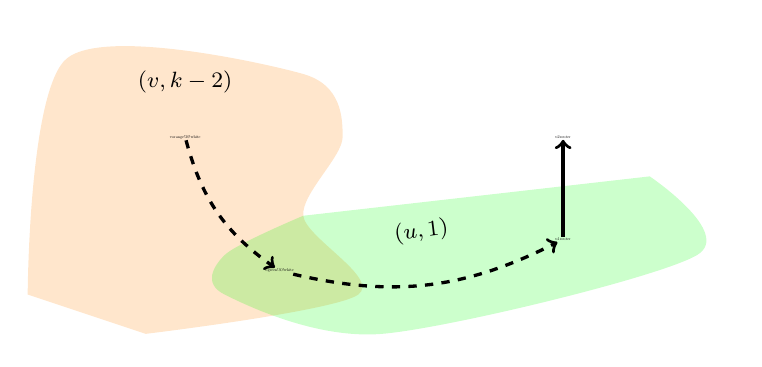
\begin{tikzpicture}

\fill[orange, opacity = 0.2] plot [smooth] coordinates { 
(-1.5, -1) 
(-1, 2) 
(2, 1.8) 
(2.5, 1) 
(2, 0) 
(2.7, -1) 
(0, -1.5)
};

\def\x{0}
\fill[green, opacity = 0.2, xscale = 2] plot [smooth] coordinates { 
(1.5-0.5+\x, 0) 
(1-0.5+\x, -0.5) 
(1-0.5+\x, -1) 
(2-0.5+\x, -1.5)
(4-0.5+\x, -0.5) 
(3.7-0.5+\x, 0.5)
};


\node[scale=0.15] (v) at (0.5, 1) {\router{v}{orange!30!white}};
\node[scale=0.15] (u) at (1.7, -0.7) {\router{u}{green!30!white}};
\node[scale=0.15] (u1) at (4.3+1, -0.3) {\router{u1}{router}};
\node[scale=0.15] (u2) at (4.3+1, -0.3+1.3) {\router{u2}{router}};

\node at (0.5, 1.7) {\footnotesize $\nreach(v, k - 2)$};
\node[rotate=7] at (3.5, -0.2) {\footnotesize $\nreach(u, 1)$};

\draw (v) edge[very thick, below, bend right=20, dashed, ->] (u);
\draw (u) edge[very thick, below, bend right=20, dashed, ->] (u1);
\draw[->, very thick] (u1) -- (u2);

%\draw (s) edge[very thick, below, bend right=10, dashed, ->] node {$\mathit{sol}(i - 1, y)$} (y);
%\draw (y) edge[very thick, bend right=10, dashed, ->, below] node {$w(y, x)$} (x);
%\draw (s) edge[very thick, bend left=40, dashed, ->, above] node {$\mathit{sol}(i - 1, x)$} (x);
%\draw (s) edge[very thick, bend right=30, dashed, ->] (z);
%\draw (z) edge[very thick, ->, sloped, below] node {$w((z, x))$} (x);
%\draw (s) edge[very thick, bend right=30, dashed, ->, below, sloped] node {$\mathit{sol}(i - 2, r)$} (r);
%\draw (r) edge[very thick, bend right=20, dashed, ->, below, sloped] node {$w(r, z)$} (z);

\end{tikzpicture}
\end{center}
\caption{Second case illustration for recurrence  of $\nreach(v, k)$}
\label{fig:nreachC2}
\end{figure}

We are now going to prove formally that the nodes discussed above cover all nodes
contained in $\nreach(v, k)$ and that both sets are the same.

\begin{theorem}
\label{thm:nreach}
Let $G$ be a network, $v \in V(G)$ and an integer $k \geq 2$. It holds that
\begin{align*}
\nreach(v, k) & = \bigcup_{u \in \nreach(v, k - 1)} \nreach(u, 1) \ \cup \\ 
& \left\{ u_2 \mid (u_1, u_2) \in E(G) \ \wedge \ \exists u \in \nreach(v, k - 2) \ u_1 \in \nreach(u, 1) \right\}
\end{align*}
\end{theorem}

\begin{proof}
Let $k \geq 2$. 

$(\subseteq)$ Suppose that $a \in \nreach(v, k)$. Then there exists a deterministic sr-path 
$\sr{p} = \langle x_1, \ldots, x_{l - 1}, x_l \rangle$ from $v$ to $a$ of segment cost at most $k$.
%Since $\sr{p}$ is deterministic, so are $\langle x_1, \ldots, x_{l - 1} \rangle$ and
%$\langle x^2_{l - 1}, x_l \rangle$.

If $x_l$ is a node segment then $\langle x_1, \ldots, x_{l - 1} \rangle$
is a deterministic sr-path of segment cost at most $k - 1$. Thus, for $u = x^2_{l - 1}$ we have
that $u \in \nreach(v, k - 1)$ and $x^2_l \in \nreach(u, 1)$. Therefore
$$
a = x^2_l \in \bigcup_{u \in \nreach(v, k - 1)} \nreach(u, 1).
$$

On the other hand, if $x_l$ is an adjacency segment then $\langle x_1, \ldots, x_{l - 1} \rangle$
is a deterministic sr-path of cost at most $k - 2$. This means that
$x^2_{l - 1} \in \nreach(v, k - 2)$. On the other hand we also have that 
$\langle x^2_{l - 1}, x_l \rangle$ is a deterministic
sr-path of cost $2$. Thus, $x^1_l \in \nreach(x^2_{l - 1}, 1)$. 
Therefore, if we write $e = x_l = (u_1, u_2)$ and $u = x^2_{l - 1}$ we have 
$x^1_l = u_1$ and
$$
(u_1, u_2) \in E(G) \ \wedge \ u \in \nreach(v, k - 2) \ \wedge \ u_1 \in \nreach(u, 1)
$$
meaning that, since $a = u_2$,
$$
a \in \left\{ u_2 \mid (u_1, u_2) \in E(G) \ \wedge \ \exists u \in \nreach(v, k - 2) \ u_1 \in \nreach(u, 1) \right\}
$$

So far we have proven that
\begin{align*}
\nreach(v, k) & \subseteq \bigcup_{u \in \nreach(v, k - 1)} \nreach(u, 1) \ \cup \\ 
& \left\{ u_2 \mid (u_1, u_2) \in E(G) \ \wedge \ \exists u \in \nreach(v, k - 2) \ u_1 \in \nreach(u, 1) \right\}
\end{align*}

$(\supseteq)$ Let $a \in \bigcup_{u \in \nreach(v, k - 1)} \nreach(u, 1)$. Then
there exists $u \in \nreach(v, k - 1)$ such that $a \in \nreach(u, 1)$. By definition,
this means that there exist deterministic sr-paths $\sr{p} = \langle x_1, \ldots, x_l \rangle$
from $v$ to $u$ with $\cost(\sr{p}) \leq k - 1$ and $\sr{q} = \langle y_1, \ldots, y_r \rangle$
from $u$ to $a$ with $\cost(\sr{q}) \leq 1$. By Lemma 
\ref{lemma:deterministic-concat} we have that $\sr{p} \oplus \sr{q}$ is a
deterministic sr-path from $v$ to $a$ of cost at most $k$. Therefore $a \in \nreach(v, k)$.

Let $a \in \left\{ u_2 \mid (u_1, u_2) \in E(G) \ \wedge \ \exists u \in \nreach(v, k - 2) \ u_1 \in \nreach(u, 1) \right\}$.
There there exists $e = (u_1, u_2) \in E(G)$ such that $u_2 = a$ and $u \in \nreach(v, k - 2)$
such that $u_1 \in \nreach(u, 1)$. By definition this means that we have a
deterministic sr-path $\sr{p}$ from $v$ to $u$ with segment cost at most $k - 2$.
Since $u_1 \in \nreach(u, 1)$ there is a unique shortest path between $u$ and $u_1$.
Therefore, $\sr{p} \oplus \langle e \rangle$ is a deterministic sr-path
from $v$ to $a$ of segment cost at most $k - 2 + 2 = k$. Hence, $a \in \nreach(v, k)$.
This concludes the proof that the right-hand side is contained in the left-hand side
so this we have equality.
\end{proof}

What we really want to compute is $\ereach(v, k)$ so we are going to see how to also
express $\ereach(v, k)$ in terms of lower values of $k$. As before, we start with the base
cases of $k = 0, 1$. When $k = 0$, only the empty path exists and it contains no edges.
Therefore $\ereach(v, 0) = \emptyset$ for all $v \in V(G)$.
For $k = 1$ we can use the same algorithm as we did for $\nreach(v, k)$ but by taking the tree
visited edges instead of the nodes as shown in Figure \ref{fig:ereach1}.

\begin{figure}[H]
\begin{center}
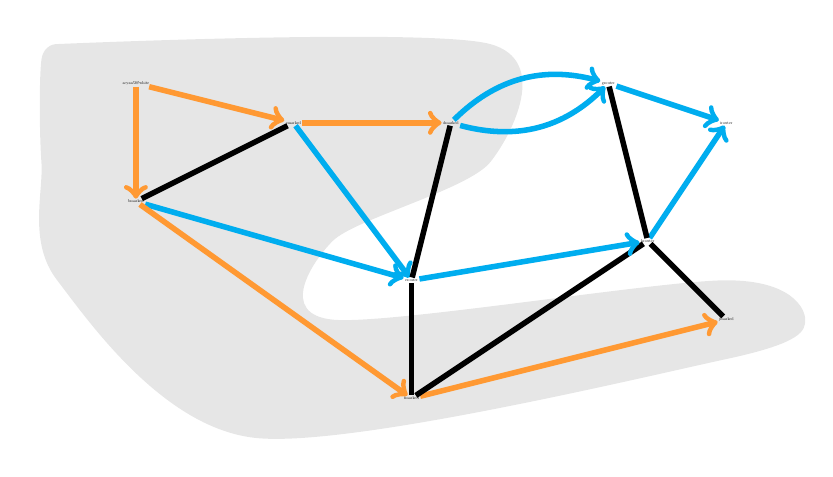
\begin{tikzpicture}
\def\x{0}
\def\y{0}

\fill[gray, opacity = 0.2] plot [smooth] coordinates { (-0.5, 1) (5, 1) (5, -0.5) (3, -1.5) (3, -2.5) (8, -2) (9, -2.5) (8, -3) (2, -4) (-0.5, -2) (-0.7, -0.5) (-0.7, 0.8) (-0.5, 1)};

\node[scale=0.15] (a) at (0.5 + \x,  0.5 + \y) {\router{a}{cyan!20!white}};
\node[scale=0.15] (b) at (0.5 + \x, -1.0 + \y) {\router{b}{marked}};
\node[scale=0.15] (c) at (2.5 + \x,  0.0 + \y) {\router{c}{marked}};
\node[scale=0.15] (d) at (4.5 + \x,  0.0 + \y) {\router{d}{marked}};
\node[scale=0.15] (e) at (4.0 + \x, -2.0 + \y) {\router{e}{router}};
\node[scale=0.15] (g) at (6.5 + \x,  0.5 + \y) {\router{g}{router}};
\node[scale=0.15] (i) at (8.0 + \x,  0.0 + \y) {\router{i}{router}};
\node[scale=0.15] (h) at (7.0 + \x, -1.5 + \y) {\router{h}{router}};
\node[scale=0.15] (f) at (4.0 + \x, -3.5 + \y) {\router{f}{marked}};
\node[scale=0.15] (j) at (8.0 + \x, -2.5 + \y) {\router{j}{marked}};
\draw[line width=2] (f) edge[above, sloped, ->, orange!80!white] node[black,font=\bfseries] {\tiny \texttt{}} (j);
\draw[line width=2] (h) edge[above, sloped] node[black,font=\bfseries] {\tiny \texttt{}} (j);
\draw[line width=2] (b) edge[above, sloped] node[black,font=\bfseries] {\tiny \texttt{}} (c);
\draw[line width=2] (c) edge[above, sloped, ->, cyan] node[black,font=\bfseries] {\tiny \texttt{}} (e);
\draw[line width=2] (b) edge[above, sloped, ->, cyan] node[black,font=\bfseries] {\tiny \texttt{}} (e);
\draw[line width=2] (b) edge[above, sloped, ->, orange!80!white] node[black,font=\bfseries] {\tiny \texttt{}} (f);
\draw[line width=2] (e) edge[above, sloped] node[black,font=\bfseries] {\tiny \texttt{}} (f);
\draw[line width=2] (h) edge[above, sloped] node[black,font=\bfseries] {\tiny \texttt{}} (f);
\draw[line width=2] (g) edge[above, sloped, ->, cyan] node[black,font=\bfseries] {\tiny \texttt{}} (i);
\draw[line width=2] (h) edge[above, sloped, ->, cyan] node[black,font=\bfseries] {\tiny \texttt{}} (i);
\draw[line width=2] (d) edge[above, sloped, bend left, ->, cyan] node[black,font=\bfseries] {\tiny \texttt{}} (g);
\draw[line width=2] (d) edge[above, sloped, bend right, ->, cyan] node[black,font=\bfseries] {\tiny \texttt{}} (g);
\draw[line width=2] (d) edge[above, sloped] node[black,font=\bfseries] {\tiny \texttt{}} (e);
\draw[line width=2] (e) edge[above, sloped, ->, cyan] node[black,font=\bfseries] {\tiny \texttt{}} (h);
\draw[line width=2] (g) edge[above, sloped] node[black,font=\bfseries] {\tiny \texttt{}} (h);
\draw[line width=2] (c) edge[above, sloped, ->, orange!80!white] node[black,font=\bfseries] {\tiny \texttt{}} (d);
\draw[line width=2] (a) edge[above, sloped, ->, orange!80!white] node[black,font=\bfseries] {\tiny \texttt{}} (b);
\draw[line width=2] (a) edge[above, sloped, ->, orange!80!white] node[black,font=\bfseries] {\tiny \texttt{}} (c);

%%%%


\end{tikzpicture}
\end{center}
\label{fig:ereach1}
\caption{$\ereach(\node{a}, 1)$ show in orange. The blue edges represent $\sp(\node{a})$.}
\end{figure}

To find a recurrence of $\ereach(v, k)$ we will proceed in the exact same way as we did for
$\nreach(v, k)$ and  explore the two situations where we extend a deterministic sr-path
with a node segment and an adjacency segment. Let $e = (u_1, u_2) \in E(G)$. If 
$e \in \ereach(u, k)$ and we can reach $u$ with a deterministic sr-path of cost
at most $k - 1$ then $e \in \ereach(v, k)$. So we have that all edges in
$$
\bigcup_{u \in \nreach(v, k - 1)} \ereach(u, 1)
$$
also belong to $\ereach(v, k)$.
We can also cover edge $e$ by using an adjacency segment on it. For this, as before, we need to
have some node $u \in \nreach(v, k - 2)$ such that $u_1 \in \nreach(u, 1)$. 
Therefore, the set
$$
\left\{ (u_1, u_2) \in E(G) \ \wedge \ \exists u \in \nreach(v, k - 2) \ u_1 \in \nreach(u, 1) \right\}.
$$
is contained in $\ereach(v, k)$.

We now prove formaly that these two sets account for all edges in $\ereach(v, k)$.

\begin{theorem}
\label{thm:ereach}
Let $G$ be a network, $v \in V(G)$ and an integer $k \geq 2$. It holds that
\begin{align*}
\ereach(v, k) & = \bigcup_{u \in \nreach(v, k - 1)} \ereach(u, 1) \ \cup \\ 
& \left\{ (u_1, u_2) \in E(G) \ \wedge \ \exists u \in \nreach(v, k - 2) \ u_1 \in \nreach(u, 1) \right\}
\end{align*}
\end{theorem}

\begin{proof}
Let $k \geq 2$. 

$(\subseteq)$ Let $e \in \ereach(v, k)$. Then there exists a deterministic sr-path 
$\sr{p} = \langle x_1, \ldots, x_{l - 1}, x_l \rangle$ from $v$ to 
$a$ of segment cost at most $k$. Moreover, either $x_l = e$ or $x_l$ is a node
segment and $e$ is the last edge of the unique shortest path between $x^2_{l - 1}$
and $x_{l}$. Let $\sr{q} = \langle x_1, \ldots x_{l - 1} \rangle$ and $u = x^2_{l - 1}$.

\emph{Case 1:} $x_l = e = (u_1, u_2)$. Let 
Since $\cost{\sr{p}} \leq k$, we know that
$\cost(\sr{q}) \leq k - 2$. Thus $u = x^2_{l - 1} \in \nreach(v, k - 2)$. 
Since $\sr{p}$ is deterministic, 
there must be a unique shortest path
between $x^2_{l - 1} = u$ to $u_1$. Therefore, $u_1 \in \nreach(u, 1)$ so
$$
e \in \left\{ (u_1, u_2) \in E(G) \ \wedge \ \exists u \in \nreach(v, k - 2) \ u_1 \in \nreach(u, 1) \right\}.
$$

\emph{Case 2:} $x_l$ is a node segment and $e$ is the last edge of the unique
shortest path between $x^2_{l - 1}$ and $x_l$. Then $\cost(\sr{q}) \leq k - 1$
so that $u \in \nreach(v, k - 1)$. Since $e$ is the last edge of the unique
shoretst path between $u = x^2_{l - 1}$ and $x_l$ we have that $e \in \ereach(u, 1)$.
Thus
$$
e \in \bigcup_{u \in \nreach(v, k - 1)} \ereach(u, 1).
$$

$(\supseteq)$ Let $e \in \bigcup_{u \in \nreach(v, k - 1)} \ereach(u, 1)$. Then
there exists $u \in \nreach(v, k - 1)$ such that $e \in \ereach(u, 1)$. By definition,
this means that there exist deterministic sr-paths $\sr{p} = \langle x_1, \ldots, x_l \rangle$
from $v$ to $u$ with $\cost(\sr{p}) \leq k - 1$ and $\sr{q}$
from $u$ to $a$ with $\cost(\sr{q}) \leq 1$ such that $e$ is the last
edge of the unique shortest path in $\sr{q}$. Thefrefore, $e \in \ereach(u, 1)$. By Lemma 
\ref{lemma:deterministic-concat} we have that $\sr{p} \oplus \sr{q} = \langle x_1, \ldots, x_r$ is a
deterministic sr-path from $v$ to $a$ of cost at most $k$. Since, $e \in \ereach(u, 1)$ and $u = x^2_{r - 1}$, 
we have that $e \in \nreach(v, k)$.

Let $(u_1, u_2) \in \left\{ (u_1, u_2) \in E(G) \ \wedge \ \exists u \in \nreach(v, k - 2) \ u_1 \in \nreach(u, 1) \right\}$.
Then there exists $u \in \nreach(v, k -2)$ such that $u_1 \in \nreach(u, 1)$. By definition this means that we have a
deterministic sr-path $\sr{p}$ from $v$ to $u$ with segment cost at most $k - 2$.
Since $u_1 \in \nreach(u, 1)$ there is a unique shortest path between $u$ and $u_1$.
Therefore, $\sr{p} \oplus \langle e \rangle$ is a deterministic sr-path
from $v$ to $a$ of segment cost at most $k - 2 + 2 = k$ with last element being an adjacency segment
on $(u_1, u_2)$. Hence, $(u_1, u_2) \in \ereach(v, k)$
\end{proof}

Given the recurrences from Theorems \ref{thm:nreach} and \ref{thm:ereach} we can easily build algorithms
for computing $\nreach(v, k)$ and $\ereach(v, k)$ for all $v$ and relevant $k$. Those are given formally as
Algorithms \ref{algo:nreach} and \ref{algo:ereach}.

\begin{algorithm}[t]
\small
\caption{$\textsf{compute-n-reach}\left( g, maxK \right)$}
\begin{algorithmic}[1]
\STATE $nreach \gets \textsf{matrix}(maxK + 1, g.\textsf{V}(), \{ \} )$
\FOR{$v \in g.\textsf{V}()$}
  \STATE $nreach(v, 0).\textsf{add}(v)$
\ENDFOR
\FOR{$v \in g.\textsf{V}()$}
  \STATE $nreach(v, 1) \gets \todo{algoV}$
\ENDFOR
\FOR{$k = 2, \ldots, maxK$}
  \FOR{$v \in g.\textsf{V}()$}
    \FOR{$u \in nreach(v, k - 1)$}
      \STATE $nreach(v, k).\textsf{or}(nreach(u, 1))$
    \ENDFOR
    \FOR{$u \in nreach(v, k - 2)$}
      \FOR{$e \in g.\textsf{E}()$}
        \STATE $nreach(v, k).\textsf{or}(\{ e.\textsf{dest}()\})$
      \ENDFOR
    \ENDFOR
  \ENDFOR
\ENDFOR
\RETURN $nreach$
\end{algorithmic}
\label{algo:nreach}
\end{algorithm}

\begin{algorithm}[t]
\small
\caption{$\textsf{compute-e-reach}\left( g, nreach \right)$}
\begin{algorithmic}[1]
\STATE $maxK \gets nreach.\textsf{nbRows}()$
\STATE $ereach \gets \textsf{matrix}(maxK + 1, g.\textsf{V}(), \{ \} )$
\FOR{$v \in g.\textsf{V}()$}
  \STATE $ereach(v, 1) \gets \todo{algoE}$
\ENDFOR
\FOR{$k = 2, \ldots, maxK$}
  \FOR{$v \in g.\textsf{V}()$}
    \FOR{$u \in nreach(v, k - 1)$}
      \STATE $ereach(v, k).\textsf{or}(ereach(u, 1))$
    \ENDFOR
    \FOR{$u \in nreach(v, k - 2)$}
      \FOR{$e \in g.\textsf{E}()$}
        \STATE $ereach(v, k).\textsf{or}(\{ e \})$
      \ENDFOR
    \ENDFOR
  \ENDFOR
\ENDFOR
\RETURN $ereach$
\end{algorithmic}
\label{algo:ereach}
\end{algorithm}


We use these algorithms to compute
$\kn(G)$ by computing $\nreach(v, k)$ until we reach some $v, k$ such that $\nreach(v, k) = V(G)$. The same holds
for the measure that we are most interested in, $\ke(G)$. We have compute $\ke(G)$ for each topology $G$ in our
data set to get a lower bound on the number of segments that are necessary to cover each network from a single vantage point.
Note that this is a lower bound since this give the number of segments to cover the network with paths, not cycles.
Figure \ref{fig:ke} shows the percentage of topologies for each value of $\ke(G)$. We see that on $90\%$ of topologies the topologies
$\ke(G) \leq 4$. Routers can often support this number of segments so we can expet that on these topologies we will be able to
implement our network monitoring solution. However some topologies exhibit a higher value of $\ke(G)$. To try to provide a solution
with a lower number of segments on such topologies we propose to compute a new set of IGP weights with a lower value of $\ke$ 
and use a monitoring scheme where the traffic is forwarded with the IGP weights originally configured on the network but the monitoring probes are routed using
these new IGP weights. We discuss this solution in the next section.

\begin{figure}
\begin{center}
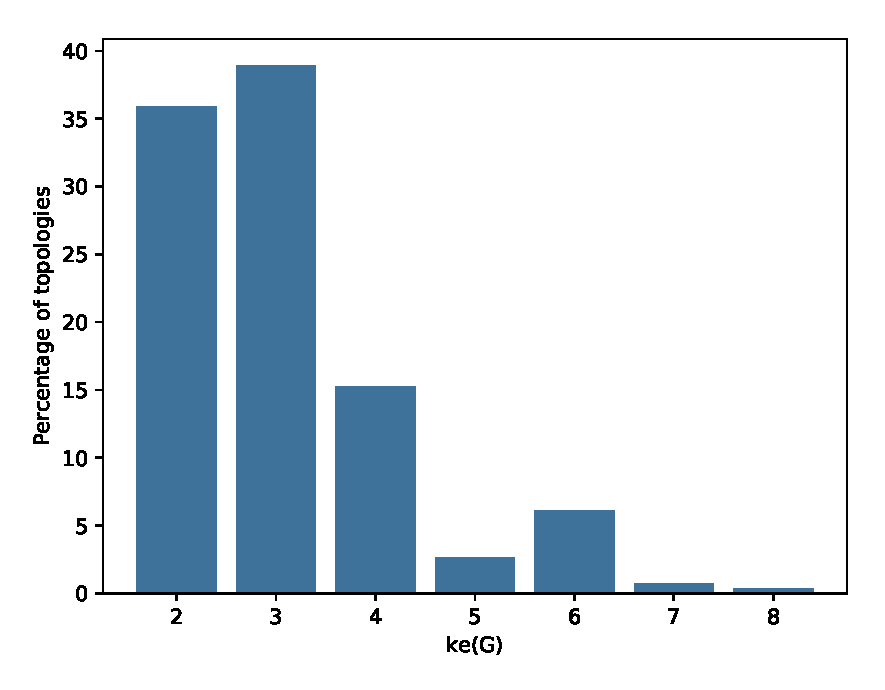
\includegraphics[width=.85\columnwidth]{./Network-lib/data/plot/edgeReach.eps}
\end{center}
\caption{Percentage of topologies for each given value of $\ke(G)$.}
\label{fig:ke}
\end{figure}


\todo{can we use this to compute and exact bound on the minimum number of segments required in any deterministic cycle cover?}


\todo{NEW INTERESTING PROBLEM: given x,y find the minimum segment cost deterministic sr-path from x to y}